\section{LoRaMAC}\label{sec:archi-loramac:proto}
\renewcommand{\rightmark}{LoRaMac}

    Cette section décris le protocole MAC mis en place pour les communications LoRa. Ce protocole est donc utilisé pour les communications entre la racine LoRa et les racines RPL. Ces dernières étant contraintes en énergie, leur radio LoRa n'est pas tout le temps allumée. Le protocole prend donc en compte cette contrainte.

\subsection{Etats d'une Racine RPL}
    Les racines RPL, utilisent 3 états (illustrés par la figure~\ref{fig:archi-state}). A l'initiation du réseau, une racine RPL se trouve dans l'état \textit{alone}. Elle demande ensuite son préfixe à la racine LoRa, et une fois celui-ci reçu, la racine RPL se trouve dans l'état \textit{ready}. Quand une racine RPL envoie une trame qui nécéssite un acquittement, tant que celui-ci n'est pas reçu elle se trouvera dans l'état \textit{wait\_response}. Une fois l'acquittement reçu, elle retournera dans l'état \textit{ready}.
    
    Les trames qui doivent être envoyées le seront en fonction de l'état dans lequel se trouve une racine RPL. Dans l'état \textit{ready}, les trames peuvent être envoyées, mais ce n'est pas le cas dans les états \textit{alone} et \textit{wait\_response}. En effet dans le premier la racine RPL ne peut pas envoyer de données car elle n'a pas encore rejoint le réseau et dans le second, elle attend un acquittement.
    \begin{figure}[H]
        \centering
        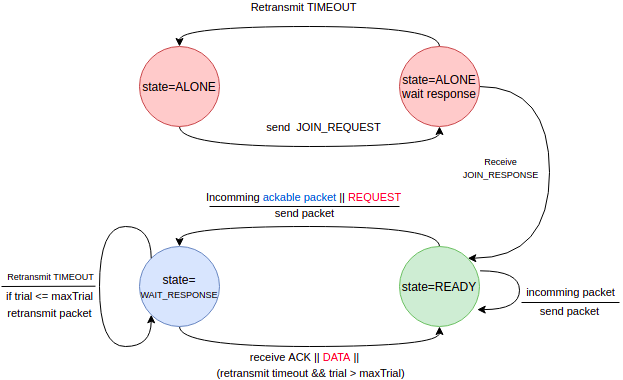
\includegraphics[scale=0.5]{res/pictures/loramac-state.drawio.png}
        \caption{Diagramme d'état des racines RPL.}
        \label{fig:archi-state}
    \end{figure}

\subsection{Construction du réseau}
    A l'initialisation du réseau, une racine RPL, doit envoyer une trame avec la commande JOIN. Une fois reçue par la racine LoRa, celle-ci va répondre avec une trame JOIN\_RESPONSE qui fait office d'acquittement de la trame JOIN et dont la payload est le préfixe IP que la racine RPL doit diffuser dans son réseau.

    Si le trame JOIN ou la trame JOIN\_RESPONSE ne sont pas reçues, la racine RPL retransmettra la trame JOIN à l'expiration d'un timer \textit{retransmit\_timer} déclanché à l'envoi de la trame JOIN. Cette se réalise tant que la réponse n'a pas été reçue.

    Une fois le préfixe reçu, la racine RPL peut initialiser le réseau RPL et y diffuser le préfixe.

\subsection{Communications montantes}
    Lorsq'un paquet est destiné à la racine LoRa, par le réseau RPL, il va remonter jusqu'à la racine RPL. Ensuite celle-ci va l'envoyer à la racine LoRa. Cette dernière a toujours sa radio allumée car elle n'est pas contrainte en énergie.

    Si la trame LoRaMAC envoyée à la racine LoRa nécéssite un acquittement, la racine RPL n'enverra pas d'autres trames tant que l'acquittement n'a pas été reçu (état \textit{wait\_response})
    à l'envoie de cette trame, le timer \textit{retransmit\_timer} est déclanché. S'il expire avant que l'acquittement ne soit reçu, la trame sera retransmise pour un maximum de 3 fois.

    Si la trame LoRaMAC envoyée à la racine LoRa ne nécéssite pas d'acquittement, la récéption ne cette trame n'est pas garantie et la racine RPL peut directement envoyé d'autres trames.

\subsection{Communications Descendantes}
    La racine LoRa possède un buffer pour chaque réseau RPL dans lesquels elle accumule les paquets corresponts au réseau RPL. Pour chaque racine RPL, lors de l'expiration, à interval régulier, du timer \textit{query\_timer}, une trame avec la commande QUERY est transmise à la racine LoRa.

    La réponse à cette trame doit être un acquittement, si la racine LoRa n'a pas de paquets pour cette racine RPL, ou une trame avec la commande DATA.

    


\subsection{Gestion des numéros de séquence}

\subsection{Evitement de collision}
